\note{Brief Overview}{
	\subsubsection*{Qualitative Application of Some Models}
	
	The three CLASP Activities in this DLM are designed to allow you to become familiar with the two models used in \hyperref[Unit1]{Unit~\ref*{Unit1}: The \ThreePhaseModel{} and the \EnergyInteractionModel{}}. The models are first applied to a substance you are very familiar with: water in its three physical phases and to a substance you are probably not familiar with: sodium acetate contained in a sealed plastic pouch, referred to as a ``heat pack.''
	
	We focus on both the physics, the physical principles and ideas contained in the models, as well as on the notion of scientific models themselves: what they are and how they are used to make sense of phenomena and how they are used to construct explanations of particular phenomena. This dual focus will be evident throughout the course. 
	
	\subsubsection*{Table copies}
	
	\begin{itemize}
		\item 2-page \ThreePhaseModel{} Summary (The two-page Model Summaries are included in the DL Workbook along with the DL CLASP Activities)
		\item 2-page \EnergyInteractionModel{} Summary
		\item Copies of each of the CLASP Activities in DLM-2
	\end{itemize}
	
	For the lead-off DL meeting that occurs immediately after lecture, make enough copies to initially have four of each per table. Ask students to leave these copies on the table at the end of the DL. After the first one or two DL section meetings on the first day following the first lecture, most students will have already purchased their DL Workbook from the Bookstore, so these table copies will no longer be necessary. In these later DLs the small number of students who don't yet have their workbook can share with other members of their small group.
	
	\subsubsection*{Equipment notes}
	
	\begin{itemize}
		\item One hotpot per table. Hotpot must have any obstruction in pour spout cut away to allow insertion of thermometers with lid tightly on.
		\item A couple of buckets of ice water (crushed ice) for cooling heat packs.
		\item Clean bottled water for use in Hotpots, with buckets for transferring water from the 5-gallon containers.
		\item Paper towels for spillage.
		\item Plastic insulating material to insulate one or two heat packs.
		\item Tongs (one per table).
	\end{itemize}
}

\note{Reminder}{
	Be a guide on the side, not a sage on the stage.
	
	The single most important thing you can do is to {\em get your students talking to each other} and {\em trying to make sense of what they are doing... }
}


\section[Making Sense of Thermal Phenomena]{Making Sense of Thermal Phenomena}
\label{act1.1.1}

\note{Timing: \unit[50]{min}}{

	\subsubsection*{Purpose}
		\begin{itemize}
			\item Provide awareness of how the thermal behavior of the heatpack differs from ordinary substances like water.
			\item Introduction to the notion of a model as the collection of ideas used to make sense of and develop explanations of particular phenomena.
			\item Provide practice using the \ThreePhaseModel{} with water.
		\end{itemize}

	\subsubsection*{Learning Outcomes}
		\begin{itemize}
			\item Be able to use the graphical representation of the \ThreePhaseModel{} to make sense of and explain why the temperature behaves the way it does when a substance such as liquid water is continuously heated.
			\item Be able to explain why there might be a difference between what a model predicts and what might actually be observed.
			\item Be able to explain how a scientific model can be used to construct an explanation of some physical phenomena such as the behavior of the temperature when adding or removing energy from a container of water.
		\end{itemize}
}

\begin{overview}

	\noindent\textbf{Overview:} We start our exploration of physics this semester by observing and reflecting on the phenomenon of ``freezing'' things.
	
\end{overview}


\subsection{Observing what happens when things freeze}

\begin{benumerate}
	\bitem{Freezing a Heat Pack}
	\todo[inline]{It would be great if we could visually offset the heading of a piece of instruction from the rest of the text, like above. I created a new \texttt{\textbackslash bitem} command, but the number is not bold. We might have to create a new enumerate environment with bold numbers to make this all look a bit better.
	
	-BH}
	\todo[inline]{I updated this enumerate environment to have bold and italicized numbering (see bracketed commands after the \texttt{\textbackslash begin\{enumerate\}} command). I can make a new environment to do this automatically if that's something we're interested in.
	
	-EH}
	\todo[inline]{This looks great, and it would be good if we could have a new environment that could do this automatically. Then we can just change the environment name instead of having to append the extra commands every time
	
	-BH}
	\todo[inline]{Done and done. The new environment is called ``benumerate'' and works just like the ``enumerate'' environment.
	
	-EH}

	
	\note{}{
		Pass out Heat Packs when you are ready for students to start after all preliminaries have been taken care of.
		Make sure students actually write something on the board. Also, make sure they write legibly and dark enough for the class to see.
	}
	
	\begin{center}
	\todo[inline]{Replace this picture with one that we actually have the rights to...}
		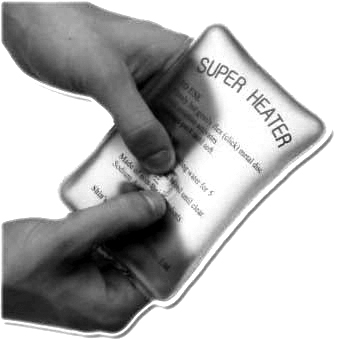
\includegraphics[width=.2\textwidth]{heatpack.jpg}
	\end{center}
	
	As a group, trigger one of the heat packs (you may know them as ``hand warmers'') on your table by clicking the button that's submerged in the liquid. Observe what happens within the heat pack during the first few minutes after triggering. Describe what you observe (i.e., tell each other a \emph{story} about what happened to the heat pack).
	
	In a few sentences, \emph{write on the whiteboard} your description (your story) of what you \textbf{\emph{observed}} (\textbf{\emph{not}} what you \emph{think} happened!). Please use words that everyone in your group is comfortable with. \textbf{Write clearly so that everybody in the room can read!}
	
	\bitem{Freezing liquid water}
	
	Based on your everyday experience, describe what you have to do to freeze water). After you have discussed this in your group for a few minutes, write your group's response on the board.
	
	\note{}{
		Desired kinds of responses something like ``put in a cold place'' or ``take heat out''
		Encourage groups to work together at board and not just have one student do all the work
	}
	
	\bitem {Does the behavior of a heat pack make sense?}
	
	Discuss in your group:
	\begin{enumerate}
		\item Based on your everyday experience with freezing things, would you say that the heat pack ``froze'' when it was triggered?
		\item Why or why not?
		\item Does the behavior of the heat pack make sense to you? Why or why not?
	\end{enumerate}
	Write your thoughts in response to (a), (b), and (c) on the whiteboard.
	\note{Possible responses}{
		\begin{enumerate}
			\item maybe/maybe not
			\item got hard and solid like ice, but didn't have to put it in a cold place. Got hotter than when a liquid.
			\item Does NOT make sense?
		\end{enumerate}
	}

\WCD

\end{benumerate}

\note{}{
	Use what students have on board to focus the summarization of the three prompts. Pick out groups to share what they have written on a particular prompt. Asking ``Why?'' and ``How do you know?'' are always good questions to ask as students present. Encourage students to speak loudly, so all can hear.
}

\subsection[Using models to make sense of physical phenomena]{Using models to make sense of physical phenomena: Introducing the \ThreePhaseModel{}}

\note{}{
	Ask students what they think of when they hear the word model. Accept all responses, but suggest confining to examples having to do with ``representing''. 

Ask students what they think a ``Scientific Model'' is.

Responses: 
Representation of certain ideas.


It is likely that any discussion of models in the first lecture didn't make much of an impression on students. Students need to get used to the idea that at one level, a model is simply the collection of ideas and relationships among those ideas, along with useful ways to represent the relationships that are needed to make sense of a particular class of phenomena, make explanations, predictions, etc. The model contains everything you need, including procedures built into the representation, that make your life much easier when doing both forefront science or responding to a quiz question.

One major goal of this first activity is to begin to get across these ideas about models. 

Intuition is good, helps us to make quick decisions and respond quickly (especially when the tiger is getting close!), but is not always so good at helping us on a quiz question. Using a model(s), on the other hand, gives you a lot of assurance that you will be on the right track (and get a good grade)

You might read the three paragraphs on the Activity Sheet to the students, have them read silently, and then summarize. However you do it, Please don't skip this part and some discussion of it.
}

\begin{reading}
\label{ReadingRefiningIntuitions}

	Before we can {\em make sense} of the process that occurs when the heat pack is triggered, we need to organize what we know about freezing and melting. You probably studied the processes of freezing and boiling in several previous science classes -- in a physical science class or chemistry in high school and perhaps in a college chemistry class. You have also had a good deal of everyday experience with freezing and boiling. But it is likely that your knowledge about these processes and phases of matter is somewhat fragmented and not well organized. Pulling together what we know and getting it organized in a useful way is what we need to do.

	\subsubsection*{{\em Learning Science} means {\em Refining Intuitions} and {\em Organizing Knowledge}}

	We all have everyday experience with lots of physical processes and phenomena. Sometimes, our intuitions seem to initially contradict the ``accepted scientific understanding.'' This is true for beginning scientists and experienced researchers alike! To continually improve our understanding of the world, we often need to refine our intuitions. In fact, we do this every day, while interacting with people, things, and situations in our environment. We use what we know about the world to make sense of our surroundings. Sometimes, we have to reorganize what we know in order to understand a new situation, and sometimes we learn something new altogether, new knowledge that we have to somehow fit in with what we already know. When this new knowledge organization becomes ``second nature'' to us, we have refined our intuition. 

	\subsubsection*{Models help scientists organize knowledge}

	One tool scientists use to organize knowledge related to a class of phenomena is the {\em scientific model}. Models bring together in one place the ideas and data patterns we use to make sense of phenomena in a concrete and useful way. A model represents these ideas in such a way that we can readily access them and use them. That is, a model typically provides the representational tools needed to use the model to develop explanations, make predictions, and more generally to make sense of phenomena. Over time, the features of a model will become second nature to us; we will have refined our intuitions about the phenomena in question.

\end{reading}

\subsubsection*{The \ThreePhaseModel{}}

	\note{}{	Probably should read this short paragraph to the class.}

	The \ThreePhaseModel{} provides a summary of the ideas needed to make sense of phase changes in matter (really, it only applies to so-called ``pure substances,'' but we won't make that distinction yet). There are instances, however, when the ``standard model'' is not sufficient to understand certain phenomena that undergo a phase change. This is the case with the heat pack. We have to extend the model, which is what we will do together in the following activities.
	

\begin{center}
\label{figTempVsEnAdd}
\begin{tikzpicture}[thick,scale=0.75, every node/.style={transform shape}]
	% title the diagram
	 \draw (7.5,7) node[align=center] {\textbf{\TempGraph{}}};

    % draw horizontal axis
    \draw[-{Stealth[scale=1.2]}, line width=1pt] (0,0) -- (14.5,0);
    % label the horizontal axis
    \draw (7.5,0) node[below=3pt] {Energy Added or Removed $\Delta E$ (at constant pressure)};

    % draw vertical axis
     \draw[-{Stealth[scale=1.2]}, line width=1pt] (0,0) -- (0,7);
    % label the vertical axis
     \draw (0,7.2) node[left=10pt, rotate=90] {Temperature $T$};
    % add melting point and boiling point on axis
     \draw[line width=1pt] (-3pt,1.8 cm) -- (3pt,1.8 cm) node[left=3pt] {\scriptsize{$T_\text{MP}$}};
     \draw[line width=1pt] (-3pt,3.8 cm) -- (3pt,3.8 cm) node[left=3pt] {\scriptsize{$T_\text{BP}$}};

	% draw first segment
	 \draw[line width=.8pt,dashed] (0,0) -- (1.5,1.8) node[below left=10pt, rotate=50.19442891] {\tiny{solid phase}};
	 
	% draw second segment
	 \draw[line width=.8pt,dashed] (1.5,1.8) -- (6,1.8) node[below left] {\tiny{mixed phase: solid/liquid}};
	 
	% draw third segment
	 \draw[line width=.8pt,dashed] (6,1.8) -- (8,3.8) node[below left=10pt, rotate=45] {\tiny{liquid phase}};

	% draw fourth segment
	 \draw[line width=.8pt,dashed] (8,3.8) -- (11.5,3.8) node[below left] {\tiny{mixed phase: liquid/gas}};

	% draw fifth segment
	 \draw[line width=.8pt,dashed] (11.5,3.8) -- (14,6.5) node[below left=10pt, rotate=47.20259816] {\tiny{gas phase}};
	 
	% draw labels
	 \draw[{Stealth[scale=.8]}-, line width=.4pt] (1.5,1.8) -- (1,2.8) node[above,align=center] {\tiny{All solid at $T_\text{MP}$}};
	 \draw[{Stealth[scale=.8]}-, line width=.4pt] (6,1.8) -- (5.5,2.8) node[above,align=center] {\tiny{All liquid at $T_\text{MP}$}};
	 \draw[{Stealth[scale=.8]}-, line width=.4pt] (8,3.8) -- (7.5,4.8) node[above,align=center] {\tiny{All liquid at $T_\text{BP}$}};
	 \draw[{Stealth[scale=.8]}-, line width=.4pt] (11.5,3.8) -- (11,4.8) node[above,align=center] {\tiny{All gas at $T_\text{BP}$}};
\end{tikzpicture}
\end{center}


%	\begin{center}
%		\label{figTempVsEnAdd}
%		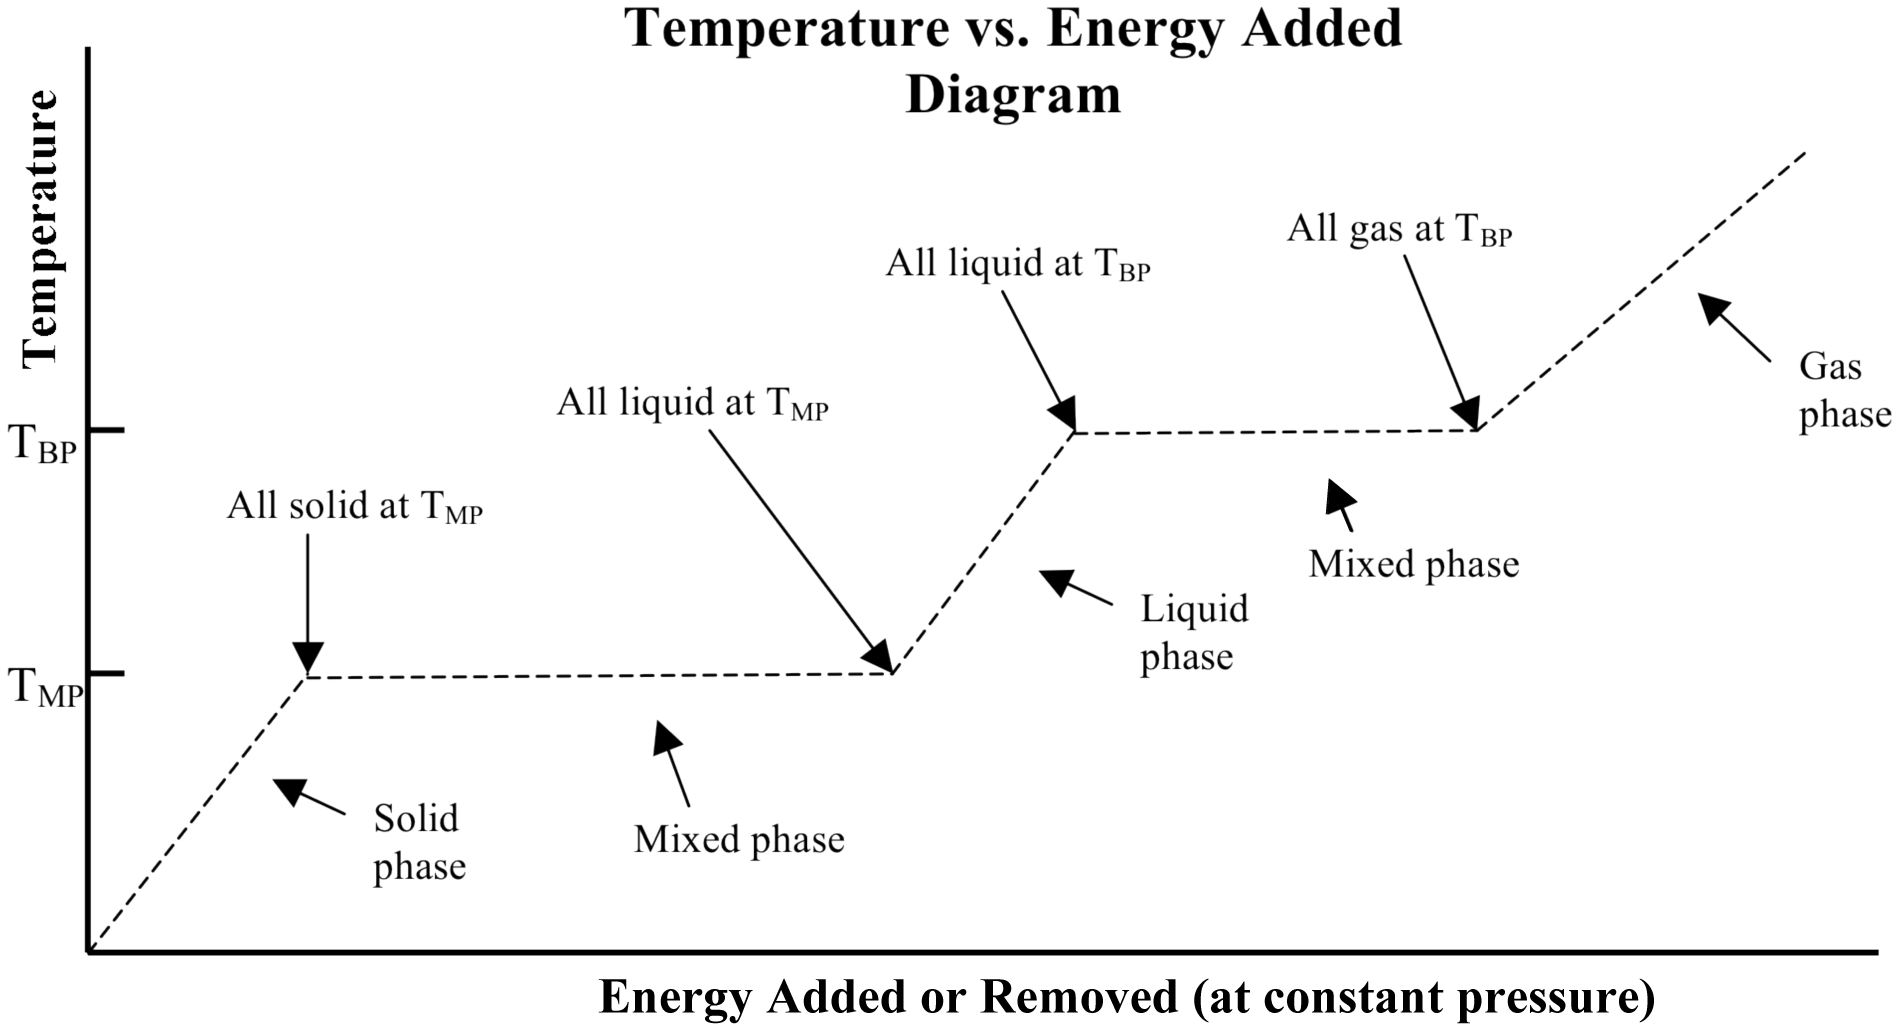
\includegraphics[width=.6\textwidth]{threephasemodel.png}
%	\end{center}

\begin{benumerate}
	\bitem {Examine the \ThreePhaseModel{} Summary}
		
	There should be several copies of the model summary sheet on your table. You can also find this summary in the online resources. Take about five minutes to look at what is on the summary sheet. Then focus on the diagrammatic representation: The \emph{\TempGraph{}}. Discuss with your group what the axes mean.
	
	\note{}{Make sure the groups have their Model Summary Sheets out and actually answer the question regarding the axes.}
	
	\bitem {Use the \ThreePhaseModel{} to construct a general explanation}

	\begin{enumerate}
		\item Put a sketch of the complete \TempGraph{} on your whiteboard that shows all three phases. Put a large dot on the graph that would represent tap water at room temperature.
		
		\item Now with the whole group participating, have someone put their finger on the dot and the rest of the group (take turns) describing what is happening to the water (tell another story!) as it is brought to a boil in the electric hotpot on your table. The person with their finger on the dot should move her/his finger along the graph to match the description. Imagine you leave the heating pot on for five or ten minutes, but not so long that all the water boils away. Now imagine putting the pot in your freezer for an hour or so and move your finger accordingly along the cooling curve.
		
		\item Repeat (b) over and over until everyone in your group is ready to explain to the whole class what goes on as you heat a substance way up and when you cool it way down. Use the language of the \ThreePhaseModel{} in your description, and use the diagram to illustrate your explanation.

\WCD

	\end{enumerate}
	\note{}{
		\begin{enumerate}
			\item Make sure every group gets their graphs on the board.  Also, make sure they get the ``dot'' in the right place.
			\item It is really important that all students in the group participate in these activities.
			\item Make sure all students are participating and that groups are taking this seriously.
		\end{enumerate}
	}

\note{}{
	Don't skip this.  ``Randomly'' call on few individual students to illustrate various processes. They need to be using phrases such as ``when you put energy (heat) in it melts more of the ice. This is represented on the graph by moving along the lower flat portion. The temperature stays constant while this happens, because the graph is horizontal here.''

	\subsubsection*{NOTE on NOMENCLATURE}
	Without making too much of a fuss about it, encourage students to use the word ``heat'' as a verb; e.g., ``We heat the water.''  ``Energy'' is what is put into or transferred to the water, during the process of heating it up.
}

	\bitem {Prepare the experiment}
	
	Use the model (and your knowledge of freezing and boiling points of water) to make a prediction (i.e., \textbf{don't start boiling the water yet!}) about temperatures:
	
	\note{}{Tell students to plug in their hot pots, but to unplug if the water starts boiling before they get to part (d).}
	
	\begin{enumerate}
		\item The hotpot in front of you should be filled about two thirds full with water. What temperature range does the model predict for the liquid water? I.e., what temperatures can liquid water have before it freezes or boils, according to the model?
		
		\item Suppose you begin heating the water. Immediately after the water has begun to boil, what does the model predict for the temperature of the liquid water? What about after it has boiled for five minutes? Compare your initial intuition with what the model tells you the temperature absolutely must be (assuming the model is appropriate for this phenomenon).
		
		\item If the lid is kept tightly on the pot and you have one thermometer immersed in the liquid and another one just above the surface of the liquid, and the water has been boiling vigorously for several minutes, what does the model tell you about the two temperatures?

	\end{enumerate}
		
	\bitem {Do the experiment}

	\begin{enumerate}
		\item Check out the model's predictions with the hot pot and the two thermometers you have at your table. On the board make a chart and compare your predictions from part 3 with your experimental results.
		
		\item Are there issues in the design of the experiment you just performed that are not taken into account in the model?  Describe these on the board and be prepared to discuss them with the class.

	\end{enumerate}

\textbf{Remember:} Make sure your responses are legible, and that your entire group agrees with what is written on the board.

	\note{}{
		\begin{enumerate}
			\item Because it is in the liquid phase, the Model for water says it must be between 0 and 100$^\circ$C.
			\item 100$^\circ$C both immediately and five min later, since we assume it will not have boiled away yet.  Make sure they get why and how the model says this.  Our intuition often tells us that the temperature will rise above 100$^\circ$C as we continue to heat it, but if the water is in the mixed phase, it must be at 100$^\circ$C according to the model.
			\item The straight-line part of the graph tells us that the temperature will be the same as long as there is some liquid and some vapor, since we are in the mixed phase.  (We assume there is nothing but water vapor -- no air -- in the space above the water.)
			\item Tell students to plug back in.  Make sure lids are on tight to prevent air getting into the pot.  Vapor should be coming out $v_i$gorously where the thermometer goes in.  When this is the case, the vapor temp is close to 100$^\circ$C.
			\item The model assumes the vapor and the liquid are in thermal equilibrium.  This implies that there is negligible energy leaving the vapor inside the top of the pot and going to the atmosphere.
			\item You will probably need to hurry the students along.
		\end{enumerate}
	}

\WCD

\note{}{
	Resolve any discrepancies among group's responses. You can ask students to compare their response with other group's responses and point out any differences.  Come to a class consensus on any discrepancies.

	Part (e) begins to get at a subtle point that we will keep coming back to.  We can be sure of our ``answers'' in terms of what the model says.  This is the level we expect the students to achieve: understand the models sufficiently well to use them to construct explanations and make predictions with high certainty that they know what they are doing.  The harder part is knowing how well the model actually fits the experimental situation/phenomenon and not making unwarranted assumptions about what can be left out of a model or what must be put in.  For (e), the model makes a completely certain prediction that the temperature in the vapor and liquid is the same, because in the model, the assumption is that the two phases are in equilibrium.  This assumption may or may not be reasonable in a real world phenomenon.  Of course, we could develop a much more sophisticated model to more precisely predict the temperature of the vapor in the top of the hot pot, but that is not our aim here. 
}

	\bitem {What does the model say?}
	\label{Part B 3j}
	
	Use the \ThreePhaseModel{} to answer the following question:
	
	When two phases of a substance are present and in thermal equilibrium (i.e., both phases have the same temperature), what do you know with certainty about certain properties or physical conditions as they relate to that substance?

	\note{}{
		The following is NOT an intuitive notion.  But it is an important aspect of the behavior of substances as they go through phase changes.  It is also Very Apparent from the graph --- the straight line --- IF the students stop to think about what the graph means.  Many students NEVER think through what the graph means!  This is a BIG part of what we want them to learn to do.
	}
	
	Discuss in your group. How does the model representation help you answer this question?

\WCD

\end{benumerate}

\note{}{See above.}